\section{性能評価}
コンテストから提供されるテスト画像649枚に対してUltra96-V2ボード上で推論を実行した.
実行時間の評価における設定項目は以下の通りである.
\begin{description}
  \item[DPU:] B2304@200/400MHz
  \item[推論画像サイズ:] 320*640
  \item[$N$ (一度に処理する画像の数):] 130
\end{description}
\subsection{実行時間}
テスト用画像 649 枚に対する推論処理時間の平均を計測した.
はじめにシングルスレッド実装における詳細な処理時間を表 \ref{tbl:time-singlethread} に示す.

\begin{table}[h]
  \caption{シングルスレッド実装における平均処理時間} \vspace{1mm}
  \label{tbl:time-singlethread}
  \begin{center}
    \begin{tabular}{cc}
      name & elapsed time (ms) \\ \hline
      $t_{\mathrm{pre\_resize}}$    & 9.36 \\ \hline
      $t_{\mathrm{pre\_normalize}}$ & 1.98 \\ \hline
      $t_{\mathrm{pop}}$            & 0.63 \\ \hline
      $t_{\mathrm{dpu}}$            & 54.1 \\ \hline
      $t_{\mathrm{push}}$           & 1.09 \\ \hline
      $t_{\mathrm{post\_labeling}}$ & 6.93 \\ \hline
      $t_{\mathrm{post\_resize}}$   & 5.25 \\ \hline
    \end{tabular}
  \end{center}
\end{table}

シングルスレッド実装では,
前処理の平均処理時間($t_{\mathrm{pre\_resize}} + t_{\mathrm{pre\_normalize}}$)は11.3ms,
DPUによるによる推論の平均処理時間($t_{\mathrm{dpu}}$)は54.1ms,
後処理の平均処理時間($t_{\mathrm{post\_labeling}} + t_{\mathrm{post\_resize}}$)は12.2msであった.
シングルスレッド実装の推論平均処理時間はこれらの合計値,すなわち,77.7msであることが分かる.

マルチスレッド実装では,
推論平均処理時間($t_{\mathrm{inference}}$)が57.9msとなった.
処理のマルチスレッド化により約25\%の高速化を達成したことが分かる.
ここで,マルチスレッド化によるオーバーヘッド $t_\alpha$ は1.93msであった.

\subsection{実行結果}

図 \ref{estimate_result} に入力画像と推論結果,および推論結果を入力画像に合成したものの1例を示す.

\begin{figure}[h]
  \begin{center}
    \caption{推論結果}
    \begin{minipage}{0.32\hsize}
      \begin{center}
        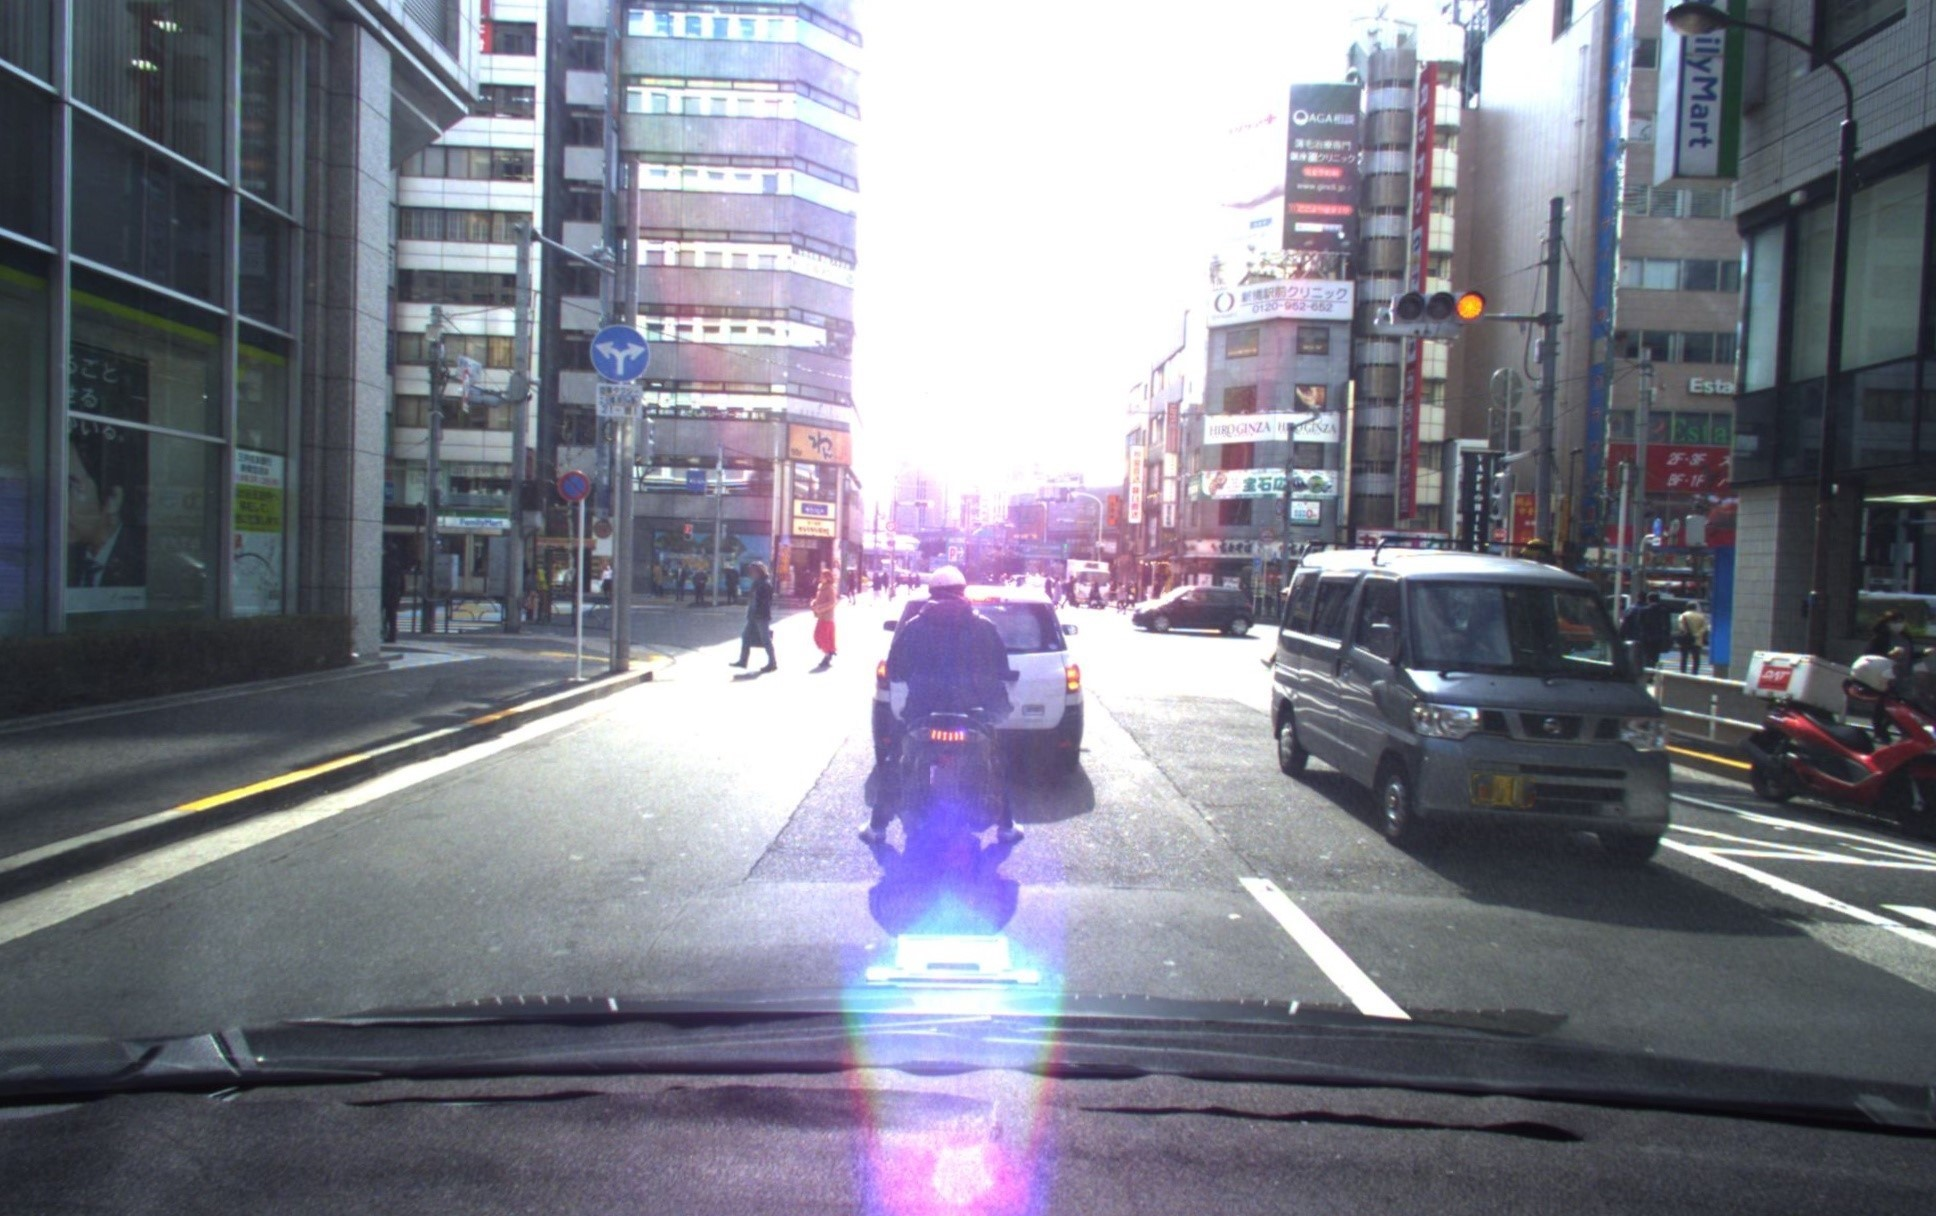
\includegraphics[width=\linewidth]{./figures/orig.jpg}
      \end{center}
    \end{minipage}
    \begin{minipage}{0.32\hsize}
      \begin{center}
        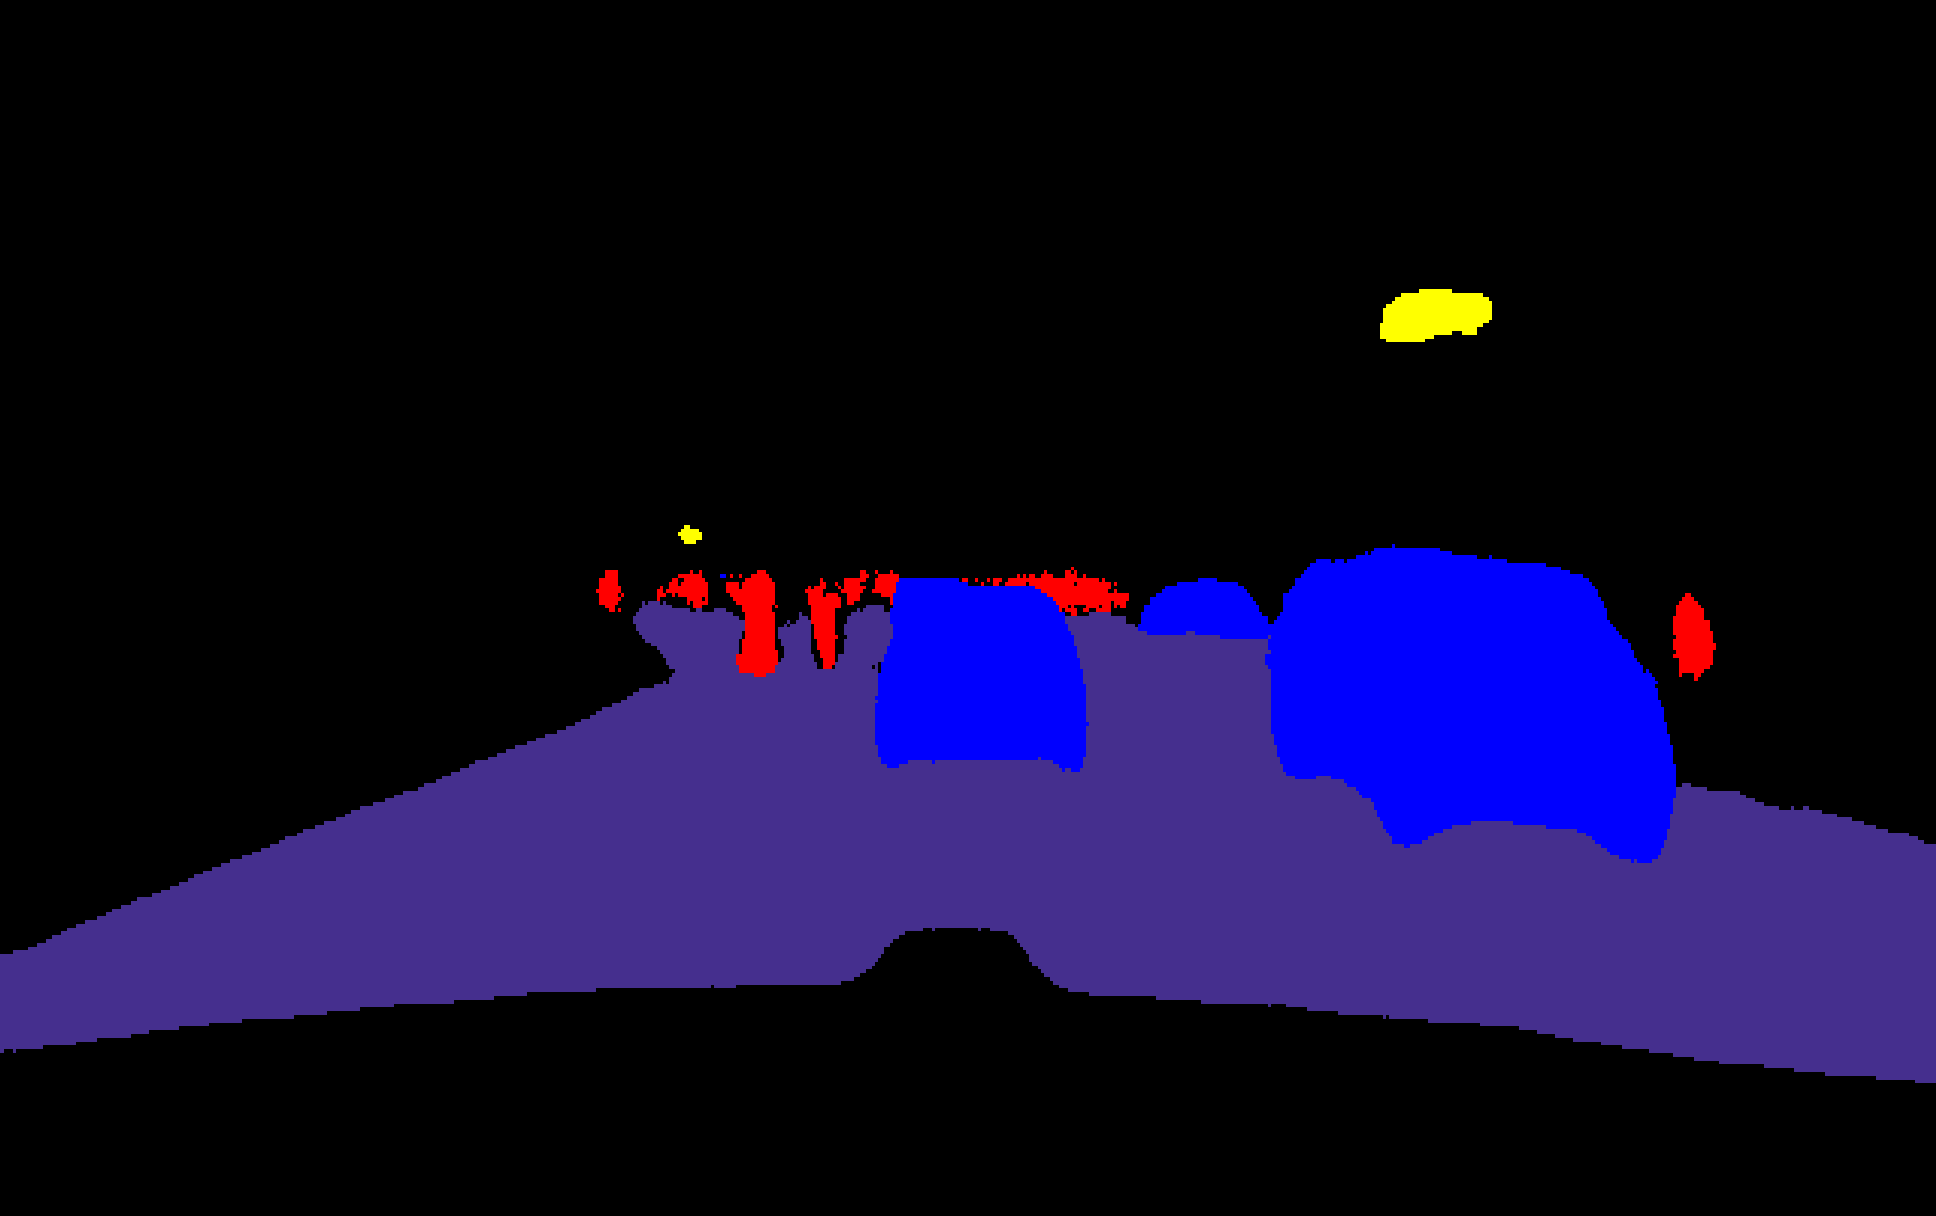
\includegraphics[width=\linewidth]{./figures/label.png}
      \end{center}
    \end{minipage}
    \begin{minipage}{0.32\hsize}
      \begin{center}
        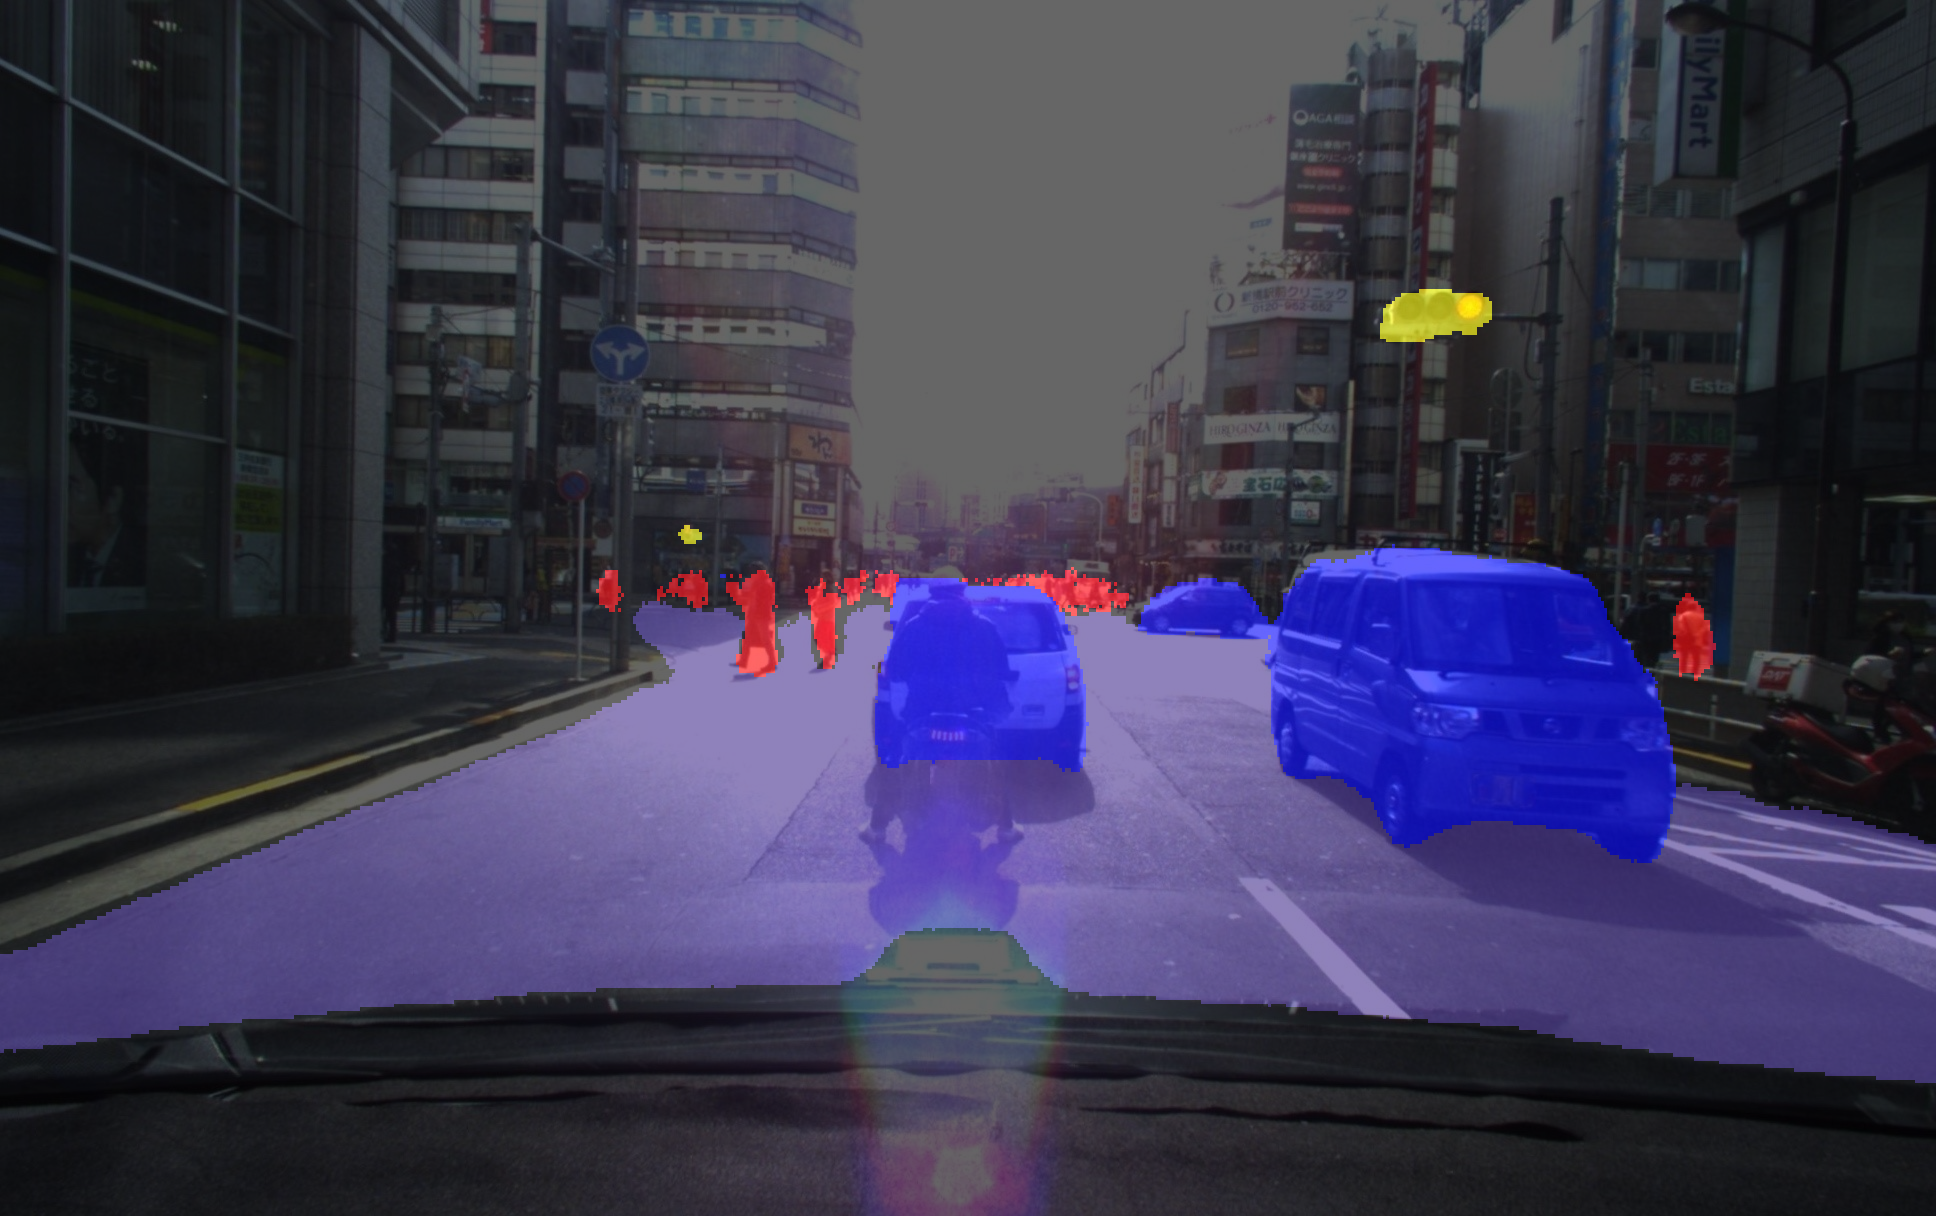
\includegraphics[width=\linewidth]{./figures/mixed.png}
      \end{center}
    \end{minipage}
    \label{estimate_result}
  \end{center}
\end{figure}
推論結果をSIGNATEに投稿した結果,mIoUスコアは0.6014857となった.

\subsection{リソース使用率}
B2304 DPUを第3章で説明したとおりのコンフィグレーションで実装した場合のDPUおよび回路全体のリソース使用率を表\ref{resource_util}に示す.
DPU IPを含んだVivadoプロジェクトをVitisが自動生成する際にベースとするプラットフォームプロジェクトにAXI GPIOやUARTなどのIPが含まれているため,今回のコンテストにおいては不要なIPも含まれている.

\begin{table}[h]
    \begin{center}
        \label{resource_util}
        \caption{リソース使用率}
        \begin{tabular}{lllllllll}
            & Total LUT & Logic LUT & LUTRAM & SRL  & FF    & RAMB36 & RAMB18 & DSP \\ \hline
        DPU & 35175     & 31982     & 1618   & 1575 & 61635 & 147    & 29     & 290 \\ \hline
        ALL & 50414     & 45964     & 2450   & 2000 & 80647 & 151    & 29     & 290
        \end{tabular}
    \end{center}
\end{table}
\subsection{消費電力}
Ultra96V2ボードに供給されるDC電源プラグに流れる電流から,消費電力を計測した.
計測値はアイドル時9.49W,推論時平均11.52W,推論時ピーク12.27Wとなった.
